\section{\sys design}
\label{sec:design}

In this section, we describe our \sys protocols. We first describe the privacy
protocol (Figure~\ref{fig:privacy}) that achieves TAP privacy and action service
privacy. Then, we describe the anonymity protocol (Figure~\ref{fig:anonymity})
that achieves recipe anonymity.

\subsection{Privacy protocol}
\label{sec:privacy}

\begin{figure}
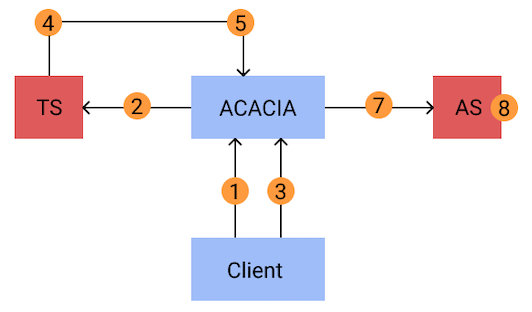
\includegraphics[width=8cm]{graphics/ACACIA.png}
\caption{\textbf{Privacy protocol flow:} (1) Recipe
  installation, (2) send encrypted recipe information, (3) generate and send
  garbled circuits, (4) get trigger data $x_t$ and execute $p(x_t, c_t)$, (5)
  send garbled inputs for computation of $f(x_t, c_t)$, (6) execute $f(x_t,
  c_a)$ in MPC, (7) send encrypted output $y$, (8) decrypt $y$ to get action
  data.}
\label{fig:privacy}
\end{figure}

\paragraph{Setup.}
Each trigger service $t \in [T]$ has a private-public key pair $(\skt_t,
\pkt_t)$ and each action service $a \in [A]$ has a private-public key pair
$(\ska_a, \pka_a)$.

\paragraph{Recipe installation.}
To set up a recipe on the TAP, the client specifies the following through the
trusted mobile client:
\begin{itemize}
  \item a trigger service $t \in [T]$, a predicate $p \in \mathbf{P}_t$, and a
    trigger constant $c_t \in \mathcal{C}$;
  \item an action service $a \in [A]$, a transformation $f \in \mathbf{T}_a$,
    and an action constant $c_a \in \mathcal{C}$.
\end{itemize}
The mobile client encrypts and sends the predicate $p$ and trigger constant
$c_t$ to the trigger service $t$ using its public key $\pkt_t$. The trigger
service can decrypt this information using its secret key $\skt_t$.

\paragraph{Garbled circuit generation.}
Since the trusted mobile client cannot send the action constant $c_a$ to the TAP
in the clear for the computation of $f(x_t, c_a)$, the client periodically
generates garbled circuits for the transformation, which then allows $y = f(x_t,
c_a)$ to be computed without the TAP learning $x_t$ or $c_a$. Importantly, the
output $y$ must be encrypted under the action service's public key $\pka_a$, so
that the action service can decrypt the result using its secret key $\ska_a$.

\paragraph{Recipe execution.}
When the trigger service $t$ receives trigger data $x_t \in \mathcal{X}$, it
executes $p(x_t, c_t)$. If the result is 1, it encodes its input $x_t$ to the
TAP in order to compute $f(x_t, c_a)$ using MPC. Otherwise, the trigger service
sends nothing. When the TAP receives the encoded input, it computes $f(x_t,
c_a)$ using MPC and sends the encrypted result to the action service $a$. The
action service $a$ decrypts to recover the action data, and then performs its
action.

\subsection{Anonymity protocol}
While the above protocol achieves TAP privacy and action service privacy, the
TAP still learns the recipes a client installs along with the trigger and action
services it uses. Here, we describe an anonymity protocol that addresses this
leakage.

\begin{figure}
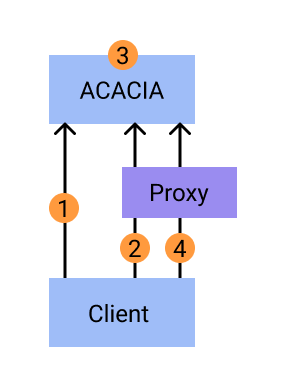
\includegraphics[height=8cm]{graphics/Proxy1.png}
\caption{\textbf{Anonymous protocol flow:} (1) Get anonymous tokens, (2) send
  recipe installation data with anonymous token, (3) check token validity and
  install recipe if valid, (4) upload garbled circuits with authorization
  token. The rest of the steps follow the privacy protocol
  (Figure~\ref{fig:privacy}).}
\label{fig:anonymity}
\end{figure}

\paragraph{Anonymous recipe installation.} In order to achieve recipe anonymity,
clients first need a way to install recipes anonymously. The main cryptographic
tool we use is an anonymous token. This allows the TAP to issue tokens that
authorize clients to install recipes. When the client later wishes to install a
recipe anonymously, it does so through an anonymity proxy (e.g., Tor) by
presenting the required recipe installation data along with an anonymous
token. Importantly, the redemption of this token cannot be linked backed to its
issuance, so the TAP cannot learn who it initially issued this token to.

\paragraph{Anonymous garbled circuit generation.}
Similar to anonymous recipe installation, clients upload garbled circuits
anonymously through the anonymity proxy and present an anonymous token that
authorizes the client to upload garbled circuits for a particular recipe.

\paragraph{Anonymous recipe execution.} Recipes execute as in the privacy
protocol, since the garbled circuits for MPC are already set up on the TAP.

\subsection{Security analysis}

Here, we analyze the security of our protocols.

\paragraph{TAP privacy.} For TAP privacy, the TAP should not learn $x_t$, $c_t$,
$c_a$, or the result of $f(x_t, c_a)$:
\begin{itemize}
  \item The TAP does not learn $c_t$, since it is encrypted to the trigger
    service.
  \item The TAP does not learn $x_t$ or $c_a$, since $f(x_t, c_a)$ is executed
    using MPC.
  \item The TAP does not learn the result of $f(x_t, c_a)$, since it is
    encrypted to the action service.
\end{itemize}

\paragraph{Action service privacy.} For action service privacy, the action
service should not learn $x_t$, except what can be inferred from the output of
$f(x_t, c_a)$.
\begin{itemize}
  \item The action service does not learn $x_t$, except what can be inferred
    from the output of $f(x_t, c_a)$, since the transformation is executed using
    MPC.
\end{itemize}

\paragraph{Recipe anonymity.} For recipe anonymity, the TAP should not be able to link
installed recipes to a particular client.
\begin{itemize}
  \item The TAP cannot link installed recipes to a particular client, since recipe
    installation and garbled circuit uploads are done using an anonymity proxy
    and are authorized via anonymous tokens.
\end{itemize}

